% Generated by thesis/ch7/exp2/exp2_figures.py -- do not edit by hand.
\begin{figure}[tbp]
  \centering
  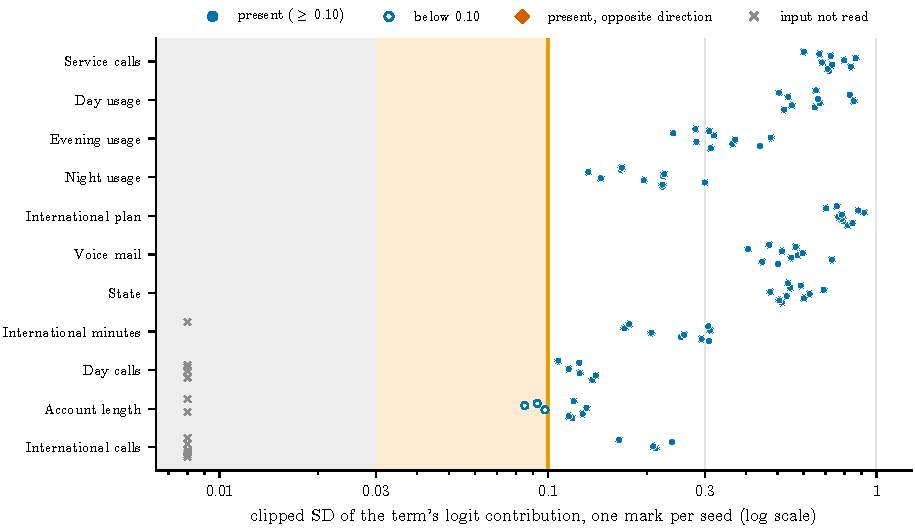
\includegraphics[width=\textwidth,height=0.8\textheight,keepaspectratio]{figures/ch7/options/lincore-churn}
  \caption{Churn: size of each linear term in each seed's network. One mark per seed (log scale). Filled blue: present ($\geq$ 0.10); open: below 0.10; red diamond: present, opposite direction to most seeds; $\times$: input not read. Shading: below 0.03 (grey) and 0.03--0.10 (orange); orange line: 0.10.}
  \label{fig:ch7-lincore-churn}
\end{figure}
